\chapter{Vector fields}
\beginlecture{15}{29.11.2024}

\section{Basics}

Let \(M\) be a smooth manifold. Recall  that we have 
\[\pi: TM \to M\]
where \(TM=\coprod_{p\in M} T_p M\). A typical point in \(TM\) is \((p,\underbrace{v}_{\in T_pM})\) and 
\[\pi((p,v))=p.\]

\begin{definition*}
    A (smooth) \dhighlight{vector field} \(X\) on \(M\) is a 
    section of \(\pi:\TM\to M\). In other words 
    \begin{enumerate}
        \item \(X:M\to TM\) smooth map 
        \item \(\pi\circ X=\text{id}\)
    \end{enumerate} 
    We let \(\mathcal{X}(M)\) be the set of vector fields on \(M\).
\end{definition*}

\dhighlight{Concretely:} To every point \(p\in M\), we associate a vector \[X(p)=X_\in T_pM.\]
Visually
\begin{figure}[H]\label{fig:7.01}
    \centering
    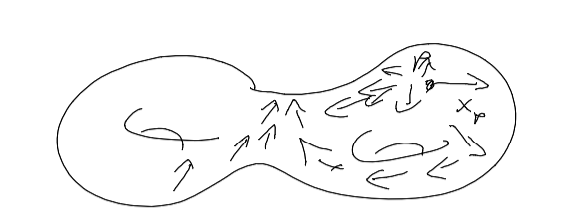
\includegraphics[width=.7\textwidth]{sketch_7_01.png}
    \caption{Sketch 7.01}
\end{figure}

Another picture:

\begin{figure}[H]\label{fig:7.02}
    \centering
    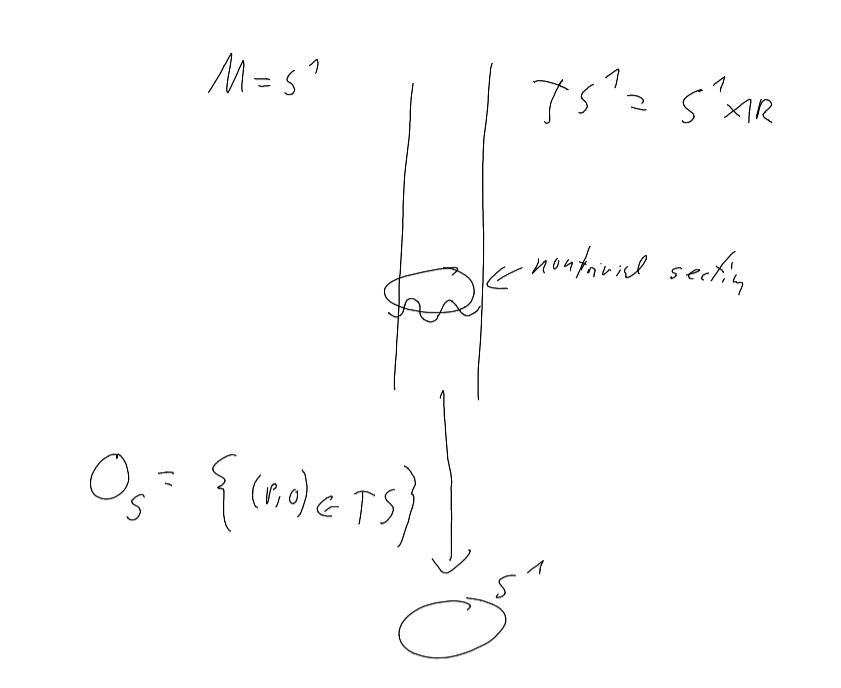
\includegraphics[width=.7\textwidth]{sketch_7_02.png}
    \caption{Sketch 7.02}
\end{figure}

\begin{lemma}\label{lem:7.1}
    \begin{enumerate} Let \(M\) be a smooth manifold.
        \item[(a)] \(\mathcal{X}(M)\) is a \(\R\) vector space 
        \item[(b)] \(\mathcal{X}(M)\) is a module over the ring \(C^{\infty}(M)\) of smooth functions on \(M\):\marginnote{\(fX(p)=\underbrace{f(p)}_{\in\R}\underbrace{X(p)}_{\in T_pM}\)}
        \[(f,X)\mapsto fX\] 
    \end{enumerate}
\end{lemma}

\begin{proof}
    Exercise.
\end{proof}

\begin{remark}\marginnote{We are not gonna study those, but it is useful to know they exist}
    In this class, we only consider smooth vector fields. If you drop the smoothness condition on the map \(X:M\to TM\),
    you get a \dhighlight{rough vector field}. 
\end{remark}

\begin{example}
    Recall that \(T_p\R^n\equiv \R^n\), hence \(T\R^n\equiv \R^n\times \R^n\).
    A vector field \(X\in\mathcal{X}(\R^n)\) is just a map  
    \begin{center}
        \begin{tikzcd}
            X:\R^n \arrow[r] & R^n\times \R^n\\
            p \arrow[r] & (p,v(p))
        \end{tikzcd}
    \end{center}
    Equivalently \(X\) is a map \(\R^n\to\R^n\), since the first coordinate is just fixed to be the 
    identity. This agrees with the notion from Analysis 2. \marginnote{A map \(\R^n\ni p\mapsto (X^1(p),\dots,X^n(p))\)}
\end{example}

\begin{remark}
    \(T_p\R^n\) has a canonical basis \(\{(\partial_{x_1})_p,\dots,(\partial_{x_n})_p\}\). This identifies 
    \((\partial_{x_i})_p\equiv (0,\dots,0,\overbrace{1}^{i\text{th component}},0\dots,0)\). We can equivalently 
    write a vector field on \(\R^n\) as \[p\mapsto (X^1(p),\dots,X^n(p))\]
    or 
    \[p\mapsto X^1(p)(\partial_{x_1})_p+\dots+X^1(p)(\partial_{x_n})_p.\]
\end{remark}

\dhighlight{Notation:} We write \(\partial_{x_i}\in\mathcal{X}(\R^n)\) for the vector field 
\[p \mapsto (\partial_{x_i})_p\in T_p\R^m\equiv (0,\dots,0,\overbrace{1}^{i\text{th component}},0\dots,0)\]
In the literature another common notation for the same thing is \(\frac{\partial}{\partial x_i}\).

\begin{example}[Vector field on \(S^3\)]
    Let \(M=\{(x_0,\dots,x_3)\mid \sum x_i^2=1\}\subset\R^{1+3}\). Let \(X=x_0\partial_{x_1}-x_1\partial_{x_0}+x_2\partial_{x_3}-x_3\partial_{x_2}\in \mathcal{X}(\R^{1+3}).\)
    Observe that \(X\perp S^3 \iff \underbrace{X\cdot v}_{X_v\cdot v} = 0, v\in S^3.\) Hence \(X \in \mathcal{X}(S^3)\).
    \begin{center}
        \begin{tikzcd}
            \arrow[d] TS^3 \arrow[r,hook] & \arrow[d,"\pi",swap] T\R^{1+3}\\
            \arrow[u,dotted,bend left,"X\restrict{S^3}"]S^3 \arrow[r,hook] & \R^{1+3}\arrow[u,bend right]
        \end{tikzcd}
    \end{center}
    where the map \(X\restrict{S^3}\) is implied by composition.
\end{example}

\begin{example}
    For any \(M\) smooth, the map \(p\mapsto 0\in T_pM\) is a vector field called the \dhighlight{zero section}.\marginnote{This is the only canonical vector field. ``There is no 1''}
\end{example}

Let \(F:M \to N\) be a smooth map. Let \(X\in\mathcal{X}(M),Y\in \mathcal{X}(N)\).

\begin{definition*}
    We say that \(X,Y\) are \(\dhighlight{\(F\)-related}\) if the following diagram commutes 
    \begin{center}
        \begin{tikzcd}
            \arrow[d]TM \arrow[r,"dF"]& TN\arrow[d] \\
            \arrow[u,bend left,"X"]M \arrow[r,"F"] & N \arrow[u,bend right,swap,"Y"] % TODO: FIX
        \end{tikzcd}
    \end{center} 
\end{definition*}

\dhighlight{Be warned!} Given \(F:M\to N, X\in\mathcal{X}(M)\), there need not exist a \(Y\in \mathcal{X}(N)\) s.t. 
\(X,Y\) are \(F\)-related. Vector fields do not push forward.\marginnote{They push back!}
\begin{figure}[H]\label{fig:7.04}
    \centering
    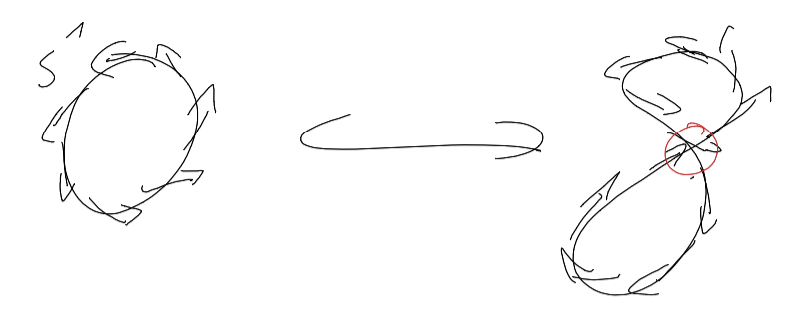
\includegraphics[width=.7\textwidth]{sketch_7_04.png}
    \caption{Sketch 7.04}
\end{figure}

\begin{definition*}
    Let \(F:M\to N\) be a diffeomorphism. Let \(X\in\mathcal{X}(M)\), we define 
    the \dhighlight{pushforward} of \(X\) \(F_\star X\in \mathcal{X}(N)\)
    by \[(F_\star X)_p=dF_{F^{-1}(p)}(X_{F^{-1}(p)}),\]
    i.e.:
    \begin{center}
        \begin{tikzcd}
            \arrow[d]TM \arrow[r,"dF"]& TN\arrow[d] \\
            \arrow[u,bend left,"X"]M  &\arrow[l,"F^{-1}"] N \arrow[u,,swap,bend right,dotted,"F_\star X"] % TODO: FIX
        \end{tikzcd}
    \end{center}
\end{definition*}

\begin{lemma}\label{7.2}
    Given \(F:M\to N\), \(G:N\to P\) diffeomorphisms, 
    \begin{enumerate}
        \item[(i)] \((G\circ F)_\star=G_\star\circ F_\star: \mathcal{X}(M)\to \mathcal{X}(P)\)
        \item[(ii)] if \(F=\text{id},M=N\), then \(F_\star=\text{id}:\mathcal{X}(M)\to \mathcal{X}(M)\)  
    \end{enumerate}
\end{lemma}

\begin{proof}
    Exercise.
\end{proof}

\section{Vector fields as derivations}

Recall: a tangent vector \(V\in T_pM\), \(p\in M\) can be viewed as a 
\dhighlight{derivation at \(p\)}, i.e. \[V:C^\infty(M)\to\R,V(fg)=f(p)V(g)+V(f)g(p).\]

\dhighlight{Notation:} Let \(X\in\mathcal{X}(M)\). Given a smooth function on \(f\in C^\infty(M)\), we 
let \(Xf\) be the map \(M\ni p\mapsto X_p f\in \R\).

\begin{lemma}\label{lem:7.3}
    \begin{enumerate}
        \item[(i)] If \(X\in \mathcal{X}(M)\), i.e. \(X\) is a smooth vector field, then \(Xf\) is a smooth function 
        \item[(ii)] Suppose that \(X:M\to TM\) is an \dhighlight{arbitrary} section (this is also known as a rough vector field). If 
                    \(Xf\) is smooth for all \(f\in C^\infty(M)\), then \(X\) is a \dhighlight{smooth} vector field.  
    \end{enumerate}
\end{lemma}

\begin{proof}
    Sheet 09. Hint: Test against coordinate functions. \marginnote{Check in \(\R^n\)}
\end{proof}

\begin{definition*}
    An \(\R\) linear map \(X:C^\infty(M)\to C^\infty(M)\) is called a \dhighlight{derivation} if, for all \(f,g\in C^\infty(M)\): 
    \[X(fg)=f\cdot Xg+Xf\cdot g\]\marginnote{The \(\cdot\) are multiplications of functions}
\end{definition*}

\begin{lemma}\label{lem:7.4}
    \begin{enumerate}
        \item If \(X\in \cX(M)\), then the map \[C^\infty(M)\ni f\mapsto Xf\in C^\infty(M)\]
              is a derivation.
        \item every derivation is of this form.
    \end{enumerate}
\end{lemma}

Upshot of the lemma: \[\cX(M)\equiv \{\text{derivations } C^\infty(M)\to C^\infty(M)\}\]
just as we identified before 
\[T_pM\equiv \{\text{derivations at } p\}.\]

\begin{proof}\marginnote{All of this follows basically by applying point wise definitions}
    (1) By definition, \(\forall p\in M\), we have 
    \begin{align*}
        X(fg)(p)=X_p(fg)&=f(p)X_pg+X_pf g(p)\\
        &= f(p)Xg(p) + Xf(p)g(p).
    \end{align*}
    Suppose that \(\nu:C^\infty\to C^\infty\) is a derivation. Define a (possibly discontinuous) 
    vector field \(X\) by setting
    \[X_pf=\underbrace{\nu f}_{\in C^\infty(M)}(p).\]
    By lemma \ref{lem:7.3} (ii) \(X\) is smooth, because \(\nu f\in C^\infty\).
\end{proof}

\begin{definition*}
    Let \(X,Y\in \mathcal{X}(M)\). We let \([X,Y]\in \cX(M)\) defined by the rule 
    \begin{equation}\label{eq:def_lie-bracket}
        C^\infty(M)\ni f\mapsto XYf-YXf \in C^\infty(M).
    \end{equation}
    We call \([X,Y]\) the \dhighlight{Lie bracket} of \(X,Y\).
\end{definition*}

\begin{lemma}\label{lem:7.5}
    Equation \ref{eq:def_lie-bracket} defines a derivation, hence \([X,Y]\)
    is a smooth vector field (by Lemma \ref{lem:7.4}). 
\end{lemma}

\begin{proof}
    For \(f,g\in C^\infty(M)\):
    \begin{align*}
        [X,Y](f,g)&=XY(fg)-YX(fg) \\
        &=X[f\cdot Yg+ Yf \cdot g]- Y [f\cdot Xg + Xf\cdot g]\\
        &=Xf\cdot Yg+f\cdot XYg+ XY f\cdot g + Xf\cdot Xg\\
        & -Yf\cdot X g- f\cdot YXg-YXf \cdot g- Xf\cdot Yg\\
        &= f(XY-YX)(g)-g(XY-YX)f \\
        &= f[X,Y]g+g[X,Y]f\qedhere 
    \end{align*}
\end{proof}

\begin{remark}[Properties of Lie bracket]
    The Lie bracket \([\cdot,\cdot]:\cX(M)\times \cX(M)\to \cX(M)\) satisfies:
    \begin{enumerate}
        \item[(i)] bilinearity: \begin{align*}
            [aX+bY,Z] &= a[X,Z]+b(Y,Z)\\
            [X,aY+bZ]&=  a[X,Y]+b(X,Z)
        \end{align*} 
        \item[(ii)] anti-symmetry \[[X,Y]=-[Y,X]\]
        \item[(iii)] Jacobi identity: \[[X,[Y,Z]]+[Y,[Z,X]]+[Z,[X,Y]]\] 
    \end{enumerate}
    Thus \((\cX(M),[\cdot,\cdot])\) is a Lie algebra (an \(\infty\)-dimensional one).
\end{remark}

\dhighlight{Warning:}

\[C^\infty(M)\ni f\mapsto XY f\in C^\infty(M)\] 
does not define a vector field in general!
\markeol{15}

\beginlecture{16}{03.12.2024}

\begin{lemma}[Naturality of Lie brackets]\label{lem:7.6}
    Given \(F:M\to N\) smooth, \(X_1,X_2\in\cX(M),Y_1,Y_2\in\cX(N)\). Assume 
    \((X_i,Y_i)\) are \(F\) related for \(i=1,2\). Then \([X_1,X_2],[Y_1,Y_2]\) are 
    \(F\)-related.
\end{lemma}

\begin{proof}
     For \(f\in C^\infty(N)\)
    \begin{align*}
        X_1X_2(f\circ F) &= X_1((Y_1f)\circ F)=(Y_1Y_2f)\circ F
    \end{align*}
    SImilarly swapping the order of \(X_1,X_2\). Hence 
    \begin{align*}
        [X_1,X_2](f\circ F)&=(X_1X_2-X_2X_1)(f\circ F)\\
        &=(Y_1Y_2-Y_2Y_1)(f)\circ F\\
        &=[Y_1,Y_2](f)\circ F\qedhere
    \end{align*}
\end{proof}

\section{Coordinate vector fields}

Let \(M\) be a smooth manifold. Let \((U,\varphi)\) be a smooth chart. 

Recall that we abuse notation by writing \(x_i\equiv x_i\circ \varphi\), where \(\underbrace{x_i}_{x^i}(x)=x_i=\pi_i(x)\).\marginnote{w.r.t the chart}
\begin{figure}[H]\label{fig:7.05}
    \centering
    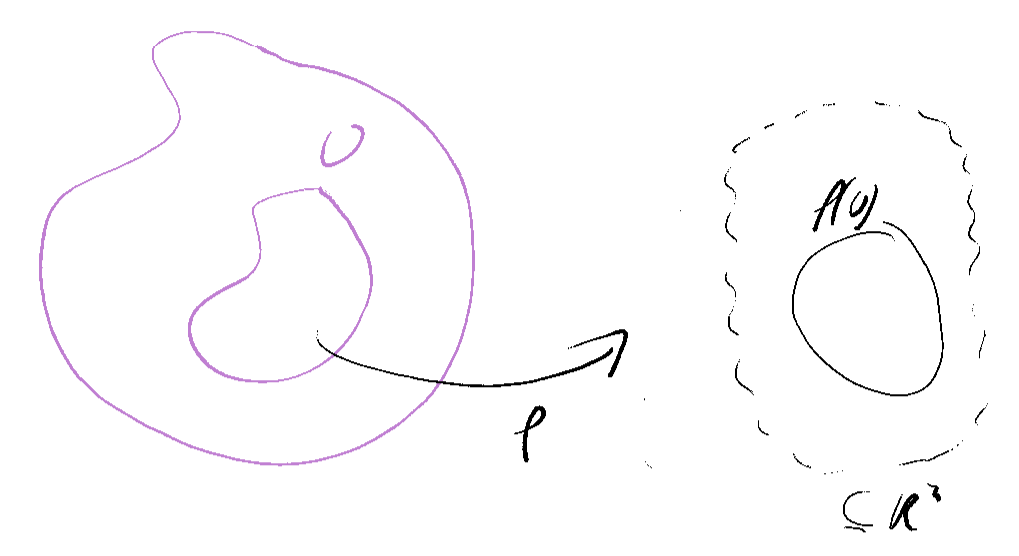
\includegraphics[width=.7\textwidth]{sketch_7_05.png}
    \caption{Sketch 7.05}
\end{figure}

If \(p\in U\), we also have been writing \((\partial_{x_i})_p=d\varphi_{\varphi(p)}^{-1}((\partial_{x_i})_{\varphi(p)})\).
\marginnote{Section of the tangent bundle, a vector field \dots}

\begin{lemma}\label{lem:7.7}
    The map \(U\ni p\mapsto (\partial_{x_i})_p\in T_p M\) is a smooth vector field on \(U\), i.e. an element 
    of \(\cX(U)\).
\end{lemma}

\begin{proof}
    Recall from last week \ref{lec15} % TODO: FIX 
    \marginnote{We often ommit the identity, i.e. the first \(n\) entries of the following} 
    \(M=\R^n\)m then the map \[(x_1,\dots,x_n)\mapsto (x_1,\dots,x_n,0,\dots,0,1,0\dots,0)\]
    Then section 7.1 % TODO 
    ,we have this is true, when \(M\) is an open subset of \(\R^n\).

    In general, \(d\varphi_{\varphi(p)}^{-1}((\partial_{x_i})_{\varphi(p)})=(\varphi)^{-1}_\star \partial_{x_i}\), where the pushfoward is 
    \[\varphi_\star^{-1}:\cX(\varphi(u))\to\cX(U).\]
    The lemma follows from the fact the fact that pushforwards of diffeomorphism send smooth vector fields to 
    smooth vector fields.
\end{proof}

\dhighlight{Notation:} The vector field \(U\ni p\mapsto (\partial_{x_i})_p\) shall be denoted by \(\partial_{x_i}\).
Other sources / authors write \(\frac{\partial}{\partial x_i}\).
\marginnote{It is important to understand the difference between vector fields and tangent vectors, like the difference between functions and elements of the target of those functions}

\begin{definition*}
    Let \(M\) be smooth of dimension \(m\).
    \begin{enumerate}
        \item[(i)] Given a point \(p\in M\), an m-tuple of vector fields \((X^1,\dots,X^m)\in \cX(M)^m\) is called a \dhighlight{local frame at \(p\)}, if \((X_p^1,\dots,X_p^m)\in T_p M^m\)\marginnote{Does this commute?
        %TODO
        }
        \item[(ii)] We say that \((X^1,\dots,X^m)\in \cX(M)^m\) is a \dhighlight{global frame} if \((X_p^1,\dots,X_p^m)\) spans \(T_pM\) for all \(p\in M\). 
    \end{enumerate}
\end{definition*}

\begin{remark}
    We take \(X^i\in \cX(M)\) and not \(\cX(U)\) for local frames, since (similar to functions), we can always extend them!
\end{remark}

\begin{lemma}\label{lem:7.8}\marginnote{This uses the fact that being full rank is an open condition}
    If \((X^1,\dots,X^m)\) is a local frame at \(p\in M\), then there exists \(p\in U\subset M\) s.t. 
    \((X^1\restrict{U},\dots,X^m\restrict{U})\in \cX(U)^m\) is a global frame on \(U\).
\end{lemma}
\begin{proof}
    Exercise using lemma \ref{lem:4.1}.
\end{proof}

\dhighlight{Key example:} If \((U,\varphi)\) is a chart on \(M\), then \((\partial_{x_1},\dots,\partial_{x_m})\in \cX(M)^m\) form 
a global frame on \(U\).

\begin{remark}[Warning]
    It is not the case that all frames are of this form, i.e. there exists frames \((X^1\dots,X^m)\in \cX(M)^m\) local frames at some 
    \(p\in M\), such that \((X^1\restrict{U},\dots,X^m\restrict{U})\) is not a coordinate vector field for any chart \((V,\psi),V\subset U\).
    E.g. \([\partial_{x_i},\partial_{x_j}]\equiv 0.\)\marginnote{It turns our the condition \([\partial_{x_i},\partial_{x_j}]\equiv 0\) is necessary and sufficient}

\end{remark}

\section{Integral curves}

Let \(\gamma:(a,b)\to M\) be a smooth map (a curve). We write 
\(\dot{\gamma}(t)=d\gamma_t(\partial_t)\in T_{\gamma(t)}M\)
\begin{center}
    \begin{tikzcd}
        \arrow[d]T\R \arrow[r,"d\gamma"]& TM\arrow[d]\\
        \arrow[u,bend left,"\partial_t"]\R \arrow[ur,dotted,"\dot{\gamma}(t)"]\arrow[r,"\gamma"] &M
    \end{tikzcd}
\end{center}

In coordinates, \(gamma(t)=(\gamma^1(t),\dots,\gamma^n(t))\in \R^n\implies \dot{\gamma}(t)=(\dot{\gamma}^1(t),\dots,\dot{\gamma}^n(t))=\gamma^1(t)\partial_{x_1}+\dots+\gamma^n(t)\partial_{x_n}\),
where \(\dot{\gamma}^i(t)=\frac{d}{dt}\gamma^i(t)\).

\begin{definition*}
    Let \(M\) be a manifold and let \(V\in \cX(M)\). An \dhighlight{integral courve} for \(V\) is a curve 
    \(\gamma:(a,b)\to M\) such that 
    \[\dot{\gamma}(t)=V_{\gamma(t)}.\]   
    We typically assume \(0\in (a,b)\), we say that the \dhighlight{starting point} \(\gamma\), is the point \(\gamma(0)\in M\).
\end{definition*}

\begin{example}
    \(M=\R^2,V=\partial_x=(1,0)\).
    \begin{figure}[H]\label{fig:7.06}
        \centering
        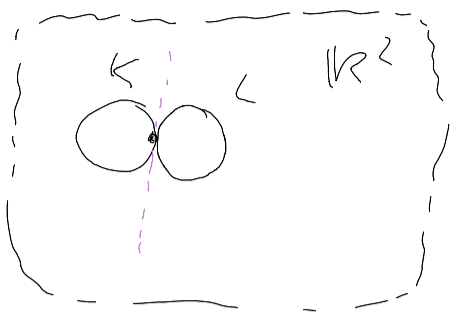
\includegraphics[width=.7\textwidth]{sketch_6_06.png}
        \caption{Sketch 7.06}
    \end{figure}
    The integral curves are precisely the curves 
    \[(t\mapsto p+t(1,0))\]
    where \(p\in \R^2\) is the starting point.
\end{example}

\begin{example}
    \(M=\R^2,V=x\partial_y-y\partial_x\equiv (-y,x)\)-
    \begin{figure}[H]\label{fig:7.07}
        \centering
        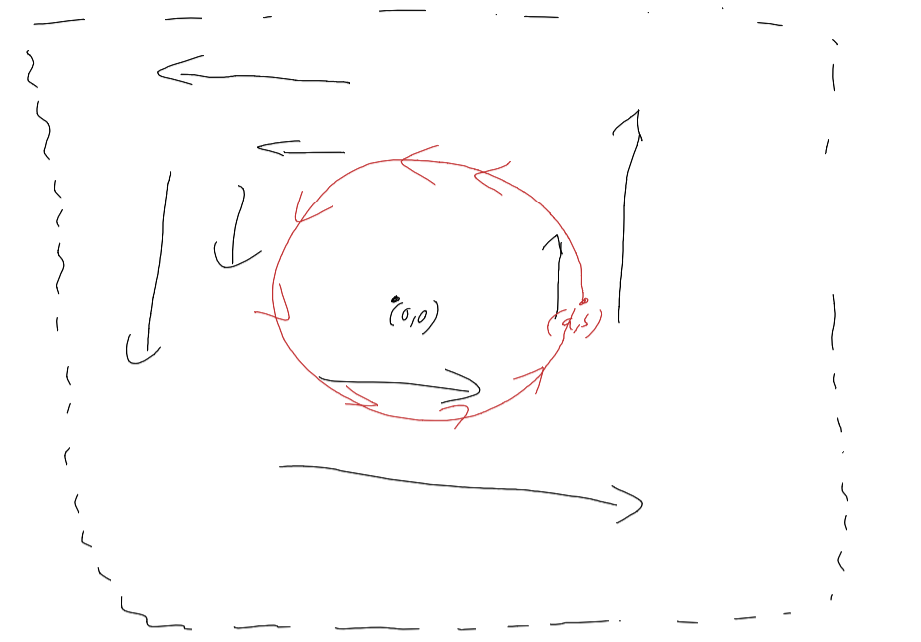
\includegraphics[width=.7\textwidth]{sketch_7_07.png}
        \caption{Sketch 7.07}
    \end{figure}

    Suppose that \(\gamma:\R\to \R^2\) is an integral curve
    \[t\mapsto (\gamma^1(t),\gamma^2(t))\]
    Then we need \begin{align*}
        \dot{\gamma}(t)&=-\gamma^2(t)\\
        \dot{\gamma}^2(t) = \gamma^1
    \end{align*}
    which is an ODE, with the following unique solution: 
    
    \begin{align*}
        \gamma^1(t)=a\cos t-b sin (t), 
        \gamma^2(t)=a \sin t + b\cos(t).
    \end{align*}
    Hence \[\gamma(t)=(a\cos t-b sin (t),a \sin t + b\cos(t))\text{, }a,b\in \R\]
    integral curve with starting point \((a,b)\).
\end{example}
%todo maybe python code and output?
\begin{proposition}\label{prop:7.9}
    Let \(M\) be a smooth manifold. Let \(V\in \cX(M)\).
    \begin{enumerate}
        \item[(a)] \dhighlight{Existence:} Given any point \(p\in M,\) there exists an open interval \(0\in J\subset \R\) and 
                   an integral curve \(\gamma:J\to M\) starting at \(p\)
        \item[(b)] \dhighlight{Uniqueness:} If \(\sigma,\gamma:J\to M\) starting at the same point \(p=\sigma(0)=\gamma(0)\), then \(\sigma=\gamma\)
    \end{enumerate}
    \begin{figure}[H]\label{fig:7.08}
        \centering
        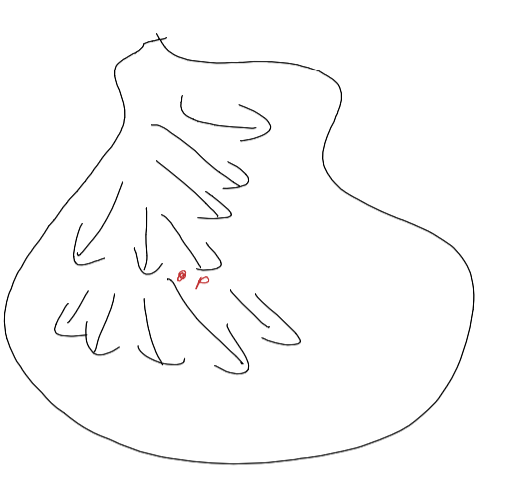
\includegraphics[width=.7\textwidth]{sketch_7_08.png}
        \caption{Sketch 7.08}
    \end{figure}
\end{proposition}

\begin{remark}\marginnote{This probably needs Zorn's lemma.}
    It follows from the proposition that,\(\forall p\in M\) there is a largest interval \(0\in J\subset\R\) admitting an integral curve \(\gamma:J\to M\).
    We call \(\gamma : J\to M\) the \dhighlight{maximal integral curve}.
\end{remark}

\begin{proof}[Proof of proposition \ref{prop:7.9}]
    (a): This is a local statement, hence we can assume open \(M\subset\R^n\). Then we must solve 
    \[\dot{\gamma}(t)=V_{\gamma(t)},\]
    \(\gamma(t)=(\gamma^1(t),\dots,\gamma^n(t))\).
    \begin{align*}
        \begin{cases}
            \dot{\gamma}^1(t)&=V^1_{\gamma(t)}\\
            \vdots & \vdots \\
            \dot{\gamma}^n(t)&=V^n_{\gamma(t)}
        \end{cases}
    \end{align*}
    This is a system of ordinary differential equations (ODEs). Hence by Theorem D.1 in the appendix of \cite{smooth_manifolds}\footnote{On the course website}, 
    the system admits a unique solution with \(\gamma(0)=p\in M \subset \R^n\). 

    (b): Let \(\mathcal{E}\subset J\) be a subset of points \(t\in J\) such that \(\sigma(t)=\gamma(t)\).\marginnote{We need this, because the uniqueness part of the theorem is local, but our statement in (b) is not}
    Observe that \(0\in\mathcal{E}\) by assumption. Observe also that \(\mathcal{E}\) is closed, since \(\sigma,\gamma\) are continuous functions.
    Moreover \(\mathcal{E}\) is open by the uniqueness part of theorem D1. \(\implies \mathcal{E}=J\).\qedhere

\end{proof}
%TODO: Citation should be in the color of the course

\begin{lemma}\label{lem:7.10}
    If \(F:M\to N,X\in \cX(M),Y\in \cX(N),X,Y\) are \(F\) related, then \(F\) takes 
    integral curves of \(X\) to integral curves of \(Y\).
\end{lemma}

\begin{proof}
    Suppose \(\gamma:J\to M\) integral curve of \(X\). 
    \begin{align*}
        (F\circ \gamma)'(t)=dF_{\gamma(t)}\dot\gamma(t)\stackrel{F\text{-related}}{=}Y_{F\circ \gamma(t)}\qedhere
    \end{align*}
\end{proof}

\begin{remark}
    There is also a converse. (exercise)
\end{remark}

\begin{definition*}
    We say that a vector field \(V\in \cX(M)\) is \dhighlight{complete} if for all 
    \(p\in M\), the maximal integral curve starting at \(p\in M\) is defined on \(\R\).
\end{definition*}

\begin{example}[Example of a non-complete vector field]
    \(M=\R\setminus\{0\},V=\partial_x\). Pick \(p=-1\in \R\). Then the integral curve starting at 
    \(p\) is the map
    \[t\mapsto -1 +t.\]
    This is only defined on \(-\infty,1\).
\end{example}


\markeol{16}



